\documentclass[tikz,border=10pt]{standalone}
\usetikzlibrary{calc}
\begin{document}
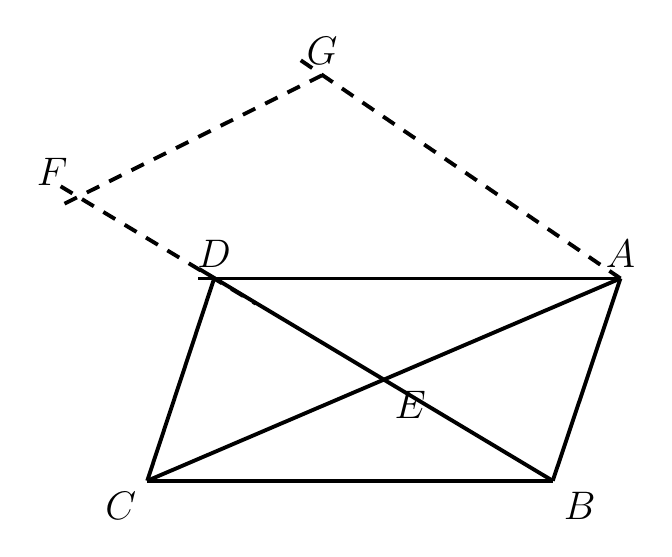
\begin{tikzpicture}[line width=1.4pt, line join=round,
  lbl/.style={font=\fontsize{15}{18}\selectfont}]
  % Vertices (pixel -> cm, s=0.01214, cx=404, cy=325)
  \coordinate (A) at (3.44,-0.05);
  \coordinate (B) at (2.58,-2.62);
  \coordinate (C) at (-2.57,-2.62);
  \coordinate (D) at (-1.72,-0.05);
  \coordinate (E) at (0.43,-1.34);
  \coordinate (F) at (-3.44,0.99);
  \coordinate (G) at (-0.35,2.53);
  % Segment end points from GES
  \coordinate (DAleft) at (-1.92,-0.05);   % D-A line start
  \coordinate (BDend) at (-1.91,0.07);     % B-D line end past D
  \coordinate (GAext) at (-0.62,2.72);     % dashed G-A beyond G
  \coordinate (FGext) at (-3.62,0.90);     % dashed F-G beyond F
  \coordinate (FDstart) at (-3.67,1.12);   % dashed F-D beyond F
  \coordinate (FDend) at (-1.19,-0.37);    % dashed F-D beyond D

  % Solid edges
  \draw[line join=round] (A) -- (C);
  \draw[line join=round] (DAleft) -- (A);
  \draw[line join=round] (C) -- (B);
  \draw[line join=round] (BDend) -- (B);
  \draw[line join=round] (D) -- (C);
  \draw[line join=round] (A) -- (B);

  % Dashed auxiliary lines
  \draw[dashed, dash pattern=on 5pt off 4pt, line join=round] (GAext) -- (A);
  \draw[dashed, dash pattern=on 5pt off 4pt, line join=round] (FGext) -- (G);
  \draw[dashed, dash pattern=on 5pt off 4pt, line join=round] (FDstart) -- (FDend);

  % Vertex labels (outside the figure)
  \node[above, lbl] at (A) {$A$};
  \node[below right, lbl] at (B) {$B$};
  \node[below left, lbl] at (C) {$C$};
  \node[above, lbl] at (D) {$D$};
  \node[below right, lbl] at (E) {$E$};
  \node[above left, lbl] at (F) {$F$};
  \node[above, lbl] at (G) {$G$};
\end{tikzpicture}
\end{document}